\section{Metodología}

\subsection{Escenario y modelo físico}
La Figura~\ref{fig:escenario} ubica el nodo sensor (Tx) y la estación de supervisión (Rx) en una bodega de unos $40\times24$~m. El camino directo tiene línea de vista; el eco modelado proviene de la cara metálica de una estantería y llega con trayectoria más larga $d_1>d_0$, ganancia compleja $\alpha=|\alpha|e^{j\varphi}$ y retardo $\tau=(d_1-d_0)/c$. Existen otras reflexiones (estantería~4), que se dejan fuera del modelo para aislar un solo mecanismo. El modelo de canal en banda base es
\begin{equation}
    r(t)=s(t)+\alpha\,s(t-\tau)+w(t), \qquad h(t)=\delta(t)+\alpha\,\delta(t-\tau),
    \label{eq:canal}
\end{equation}
cuya respuesta en frecuencia es $|H(f)|^2=|1+\alpha e^{-j2\pi f\tau}|^2$, con máximos $(1+|\alpha|)^2$ y mínimos $(1-|\alpha|)^2$ separados $1/\tau$ en frecuencia.

\textbf{Normalización del retardo.} Con los parámetros del curso, $T_s=1/R_s=31{,}25~\mu$s, lo que equivale a una diferencia de trayectorias de $cT_s\approx9{,}4$~km. En una bodega real ($\tau\sim$100~ns) se cumpliría $\tau/T_s\approx3\times10^{-3}$ y el canal sería prácticamente plano a 32~kBd. Por ello el retardo se fijó en $\tau=T_s$ (8 muestras), un modelo normalizado que reproduce la situación $\tau/T_s=1$. Esa situación se presentaría en la misma bodega si el enlace operara a decenas de MBd ($R_s\approx1/\tau=10$~MBd), sin modificar los parámetros de referencia exigidos por la guía \cite{guia1}.

\begin{figure*}[!t]
\centering
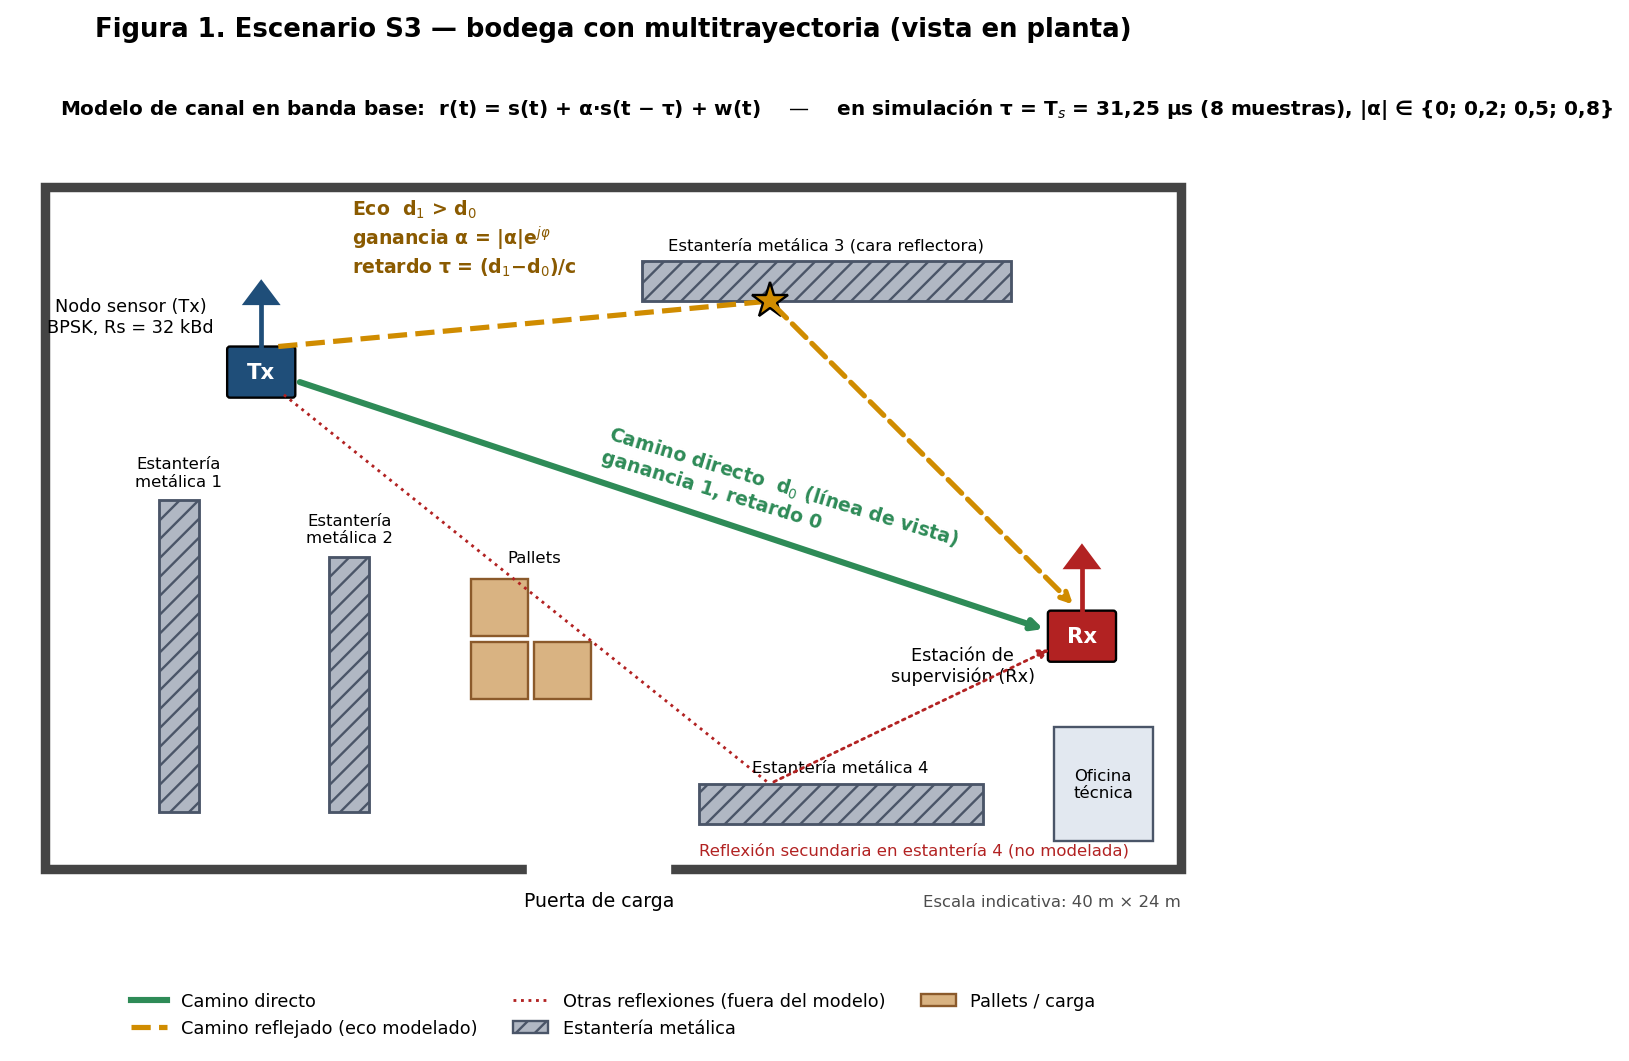
\includegraphics[width=0.78\textwidth]{Fig1_Escenario_S3_bodega.png}
\caption{Escenario S3 (imagen contextual propia): bodega con estanterías metálicas, Tx y Rx con antenas, camino directo, eco modelado y reflexión secundaria no modelada.}
\label{fig:escenario}
\end{figure*}

\subsection{Decisión de modulación y parámetros}
Se eligió BPSK ($M=2$) porque la información de telemetría es de baja tasa y conviene la máxima separación entre símbolos ($d=2$ con energía unitaria). Así, el único mecanismo de degradación observable es el eco. Se consideró QPSK, que duplica $R_b$ con la misma $R_s$, pero la cuadratura y la fase del eco mezclarían los ejes I/Q y harían más difícil atribuir la degradación al eco. Las relaciones del sistema \cite{guia1,guia2} son
\begin{align}
    k&=\log_2 M = 1~\text{bit/símbolo}, \qquad R_b=R_s\,k=32~\text{kb/s},\label{eq:rb}\\
    f_s&=R_s\cdot Sps=32\,000\times 8=256~\text{kS/s}.\label{eq:fs}
\end{align}
Con pulso rectangular de duración $T_s$, la DEP de la envolvente compleja es $S(f)\propto\mathrm{sinc}^2(fT_s)$. Su lóbulo principal ocupa $|f|<R_s$, es decir, $BW_{\text{nulo-nulo}}=2R_s=64$~kHz, con nulos en múltiplos de 32~kHz. La relación $BW\approx(1+\beta)R_s$ aplica solo a conformación RRC; se mantuvo el pulso rectangular del GRC base, como se decidió en la ficha, para no introducir ISI propia del filtro. Los 32~kb/s superan con amplitud la necesidad de variables de proceso lentas, y $Sps=8$ da resolución suficiente para el ojo y para ubicar el retardo en muestras enteras. La Tabla~\ref{tab:parametros} resume la configuración.

\begin{table}[!t]
\centering
\caption{Parámetros del sistema implementado}
\label{tab:parametros}
\footnotesize
\begin{tabular}{llc}
\toprule
\textbf{Parámetro} & \textbf{Variable GRC} & \textbf{Valor} \\
\midrule
Modulación / tabla & \texttt{tabla\_de\_verdad\_constelacion} & BPSK $(-1, +1)$ \\
Símbolos / bits por símbolo & \texttt{M}, \texttt{bps} & 2 / 1 \\
Tasa de símbolos & \texttt{Rs} & 32~kBd \\
Tasa de bits & \texttt{Rb} & 32~kb/s \\
Muestras por símbolo & \texttt{Sps} & 8 \\
Tasa de muestreo & \texttt{samp\_rate} & 256~kS/s \\
Pulso Tx / filtro Rx & \texttt{h}, \texttt{h\_mf} & $[1]\times8$ / $[1/8]\times8$ \\
Retardo del eco & \texttt{D\_eco} & 8 muestras ($31{,}25~\mu$s) \\
Ganancia del eco & \texttt{eco\_alpha}, \texttt{eco\_fase\_deg} & $\{0;0{,}2;0{,}5;0{,}8\}$, $0^\circ$ \\
AWGN de referencia & \texttt{noise\_amp} & 0,10 \\
\bottomrule
\end{tabular}
\end{table}

\subsection{Arquitectura implementada en GNU Radio}
Se partió de una copia de \texttt{Modulaciones\_basadas\_en\_constelaciones\_AWGN.grc} (Figura~\ref{fig:grc_base}), que se conservó intacta, y se creó \texttt{S3\_Multitrayectoria\_BPSK\_Grupo5.grc} (Figuras~\ref{fig:bloques} y \ref{fig:grc_mod}). Las modificaciones fueron:
\begin{itemize}
    \item \textbf{Transmisor:} tabla BPSK $(-1+0j, 1+0j)$; se conservan la fuente aleatoria, el empaquetado, el mapeo y el conformador rectangular por interpolación.
    \item \textbf{Canal S3:} \emph{Delay} de \texttt{D\_eco}$=Sps$ muestras y \emph{Multiply Const} por \texttt{alpha\_c}$=|\alpha|e^{j\varphi}$, sumados al camino directo; después se suma la fuente AWGN original. Un \emph{QT GUI Chooser} selecciona las pruebas A--D.
    \item \textbf{Receptor (Guía~2):} (1) filtro acoplado FIR $h_{mf}=[1/8]\times8$, coherente con el pulso rectangular (integrar y descargar); (2) \emph{QT GUI Eye Sink} sobre la parte real para ubicar el instante de máxima apertura; (3) \emph{Keep One in N} con $N=8$, que conserva la muestra $8k+7$, justo al final del símbolo, donde el filtro acoplado alcanza su pico (verificado numéricamente); (4) decisión con \emph{Complex to Real} y \emph{Binary Slicer} con umbral 0; (5) validación: XOR entre bits Tx retardados \texttt{delay\_bits} y bits Rx, promedio móvil de $N_{ber}=20\,000$ bits y comparación gráfica de bits.
\end{itemize}
A la salida del filtro acoplado, la muestra de decisión es
\begin{equation}
    y_k = s_k + \alpha\, s_{k-1} + n_k, \qquad \sigma_n^2=\frac{N_0R_s}{2},
    \label{eq:yk}
\end{equation}
de modo que cada punto BPSK se desdobla en $\pm1\pm\alpha$ y la distancia mínima al umbral pasa de 1 a $1-|\alpha|$.

\begin{figure}[!t]
\centering
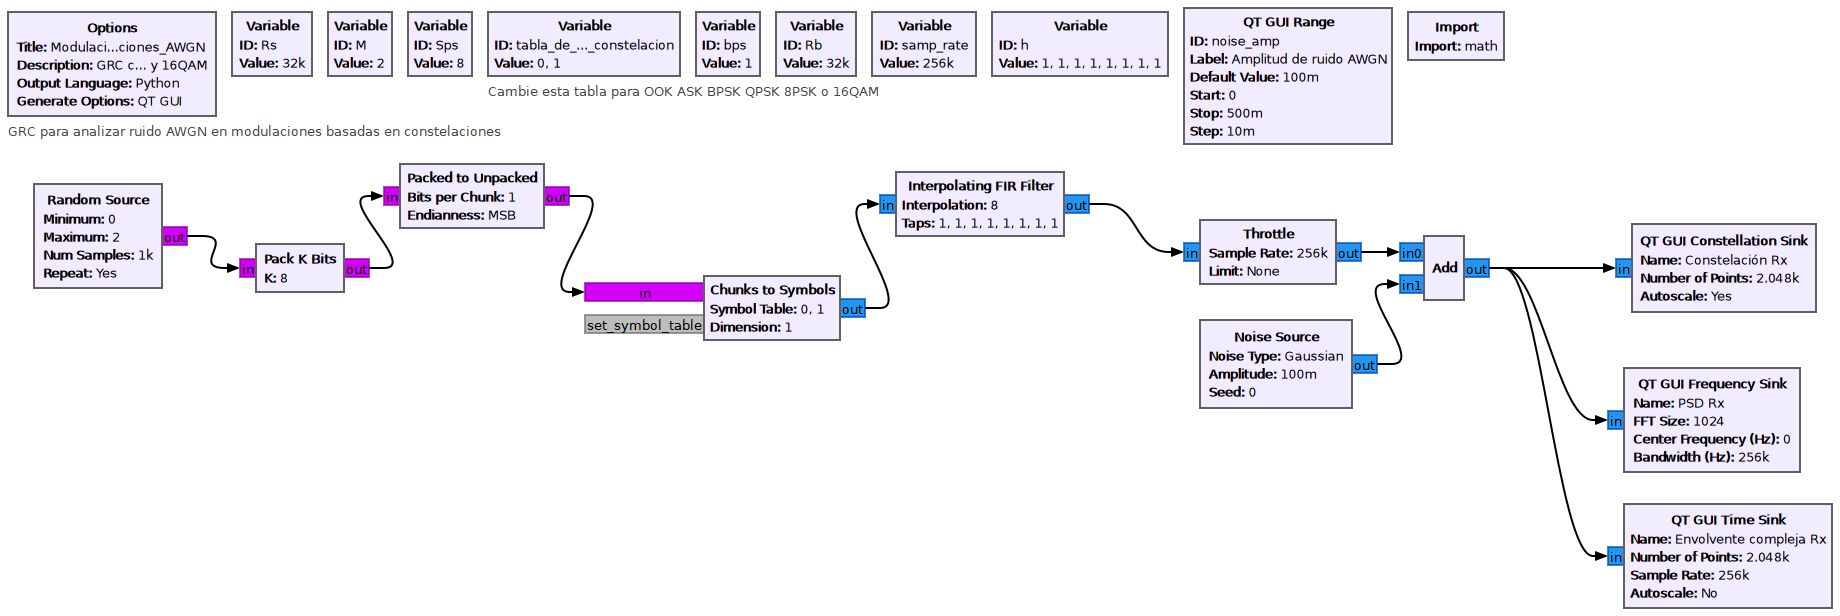
\includegraphics[width=\columnwidth]{GRC_base_original_constelaciones_AWGN.png}
\caption{GRC base del curso (\texttt{Modulaciones\_basadas\_en\_constelaciones\_AWGN.grc}), sin modificar; captura de GNU Radio Companion 3.10.12.}
\label{fig:grc_base}
\end{figure}

\begin{figure*}[!t]
\centering
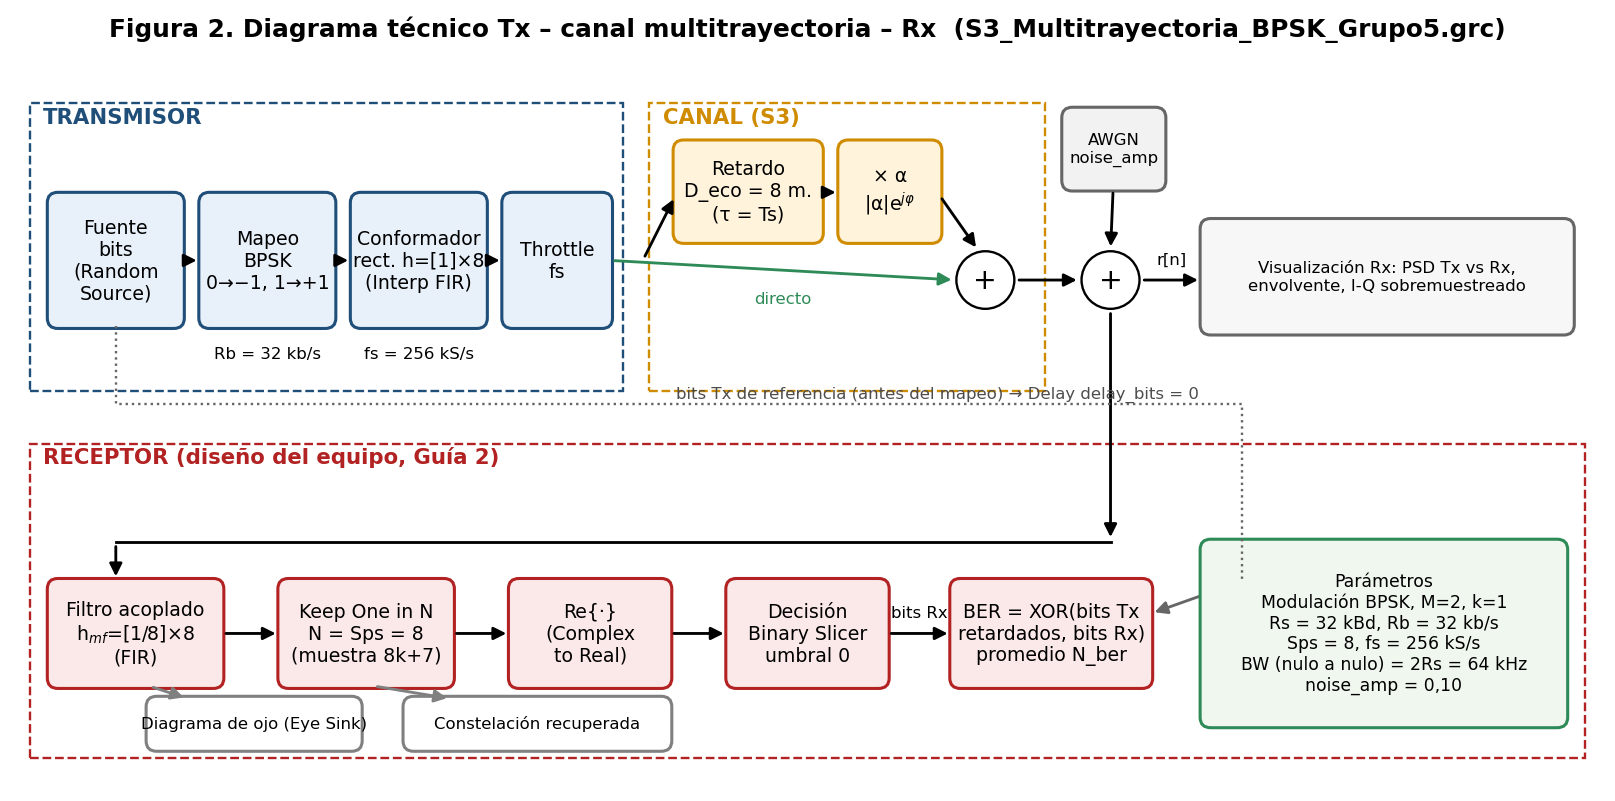
\includegraphics[width=0.92\textwidth]{Fig2_Diagrama_Tx_Canal_Rx.png}
\caption{Diagrama técnico del sistema Tx -- canal multitrayectoria -- Rx con sus parámetros.}
\label{fig:bloques}
\end{figure*}

\begin{figure*}[!t]
\centering
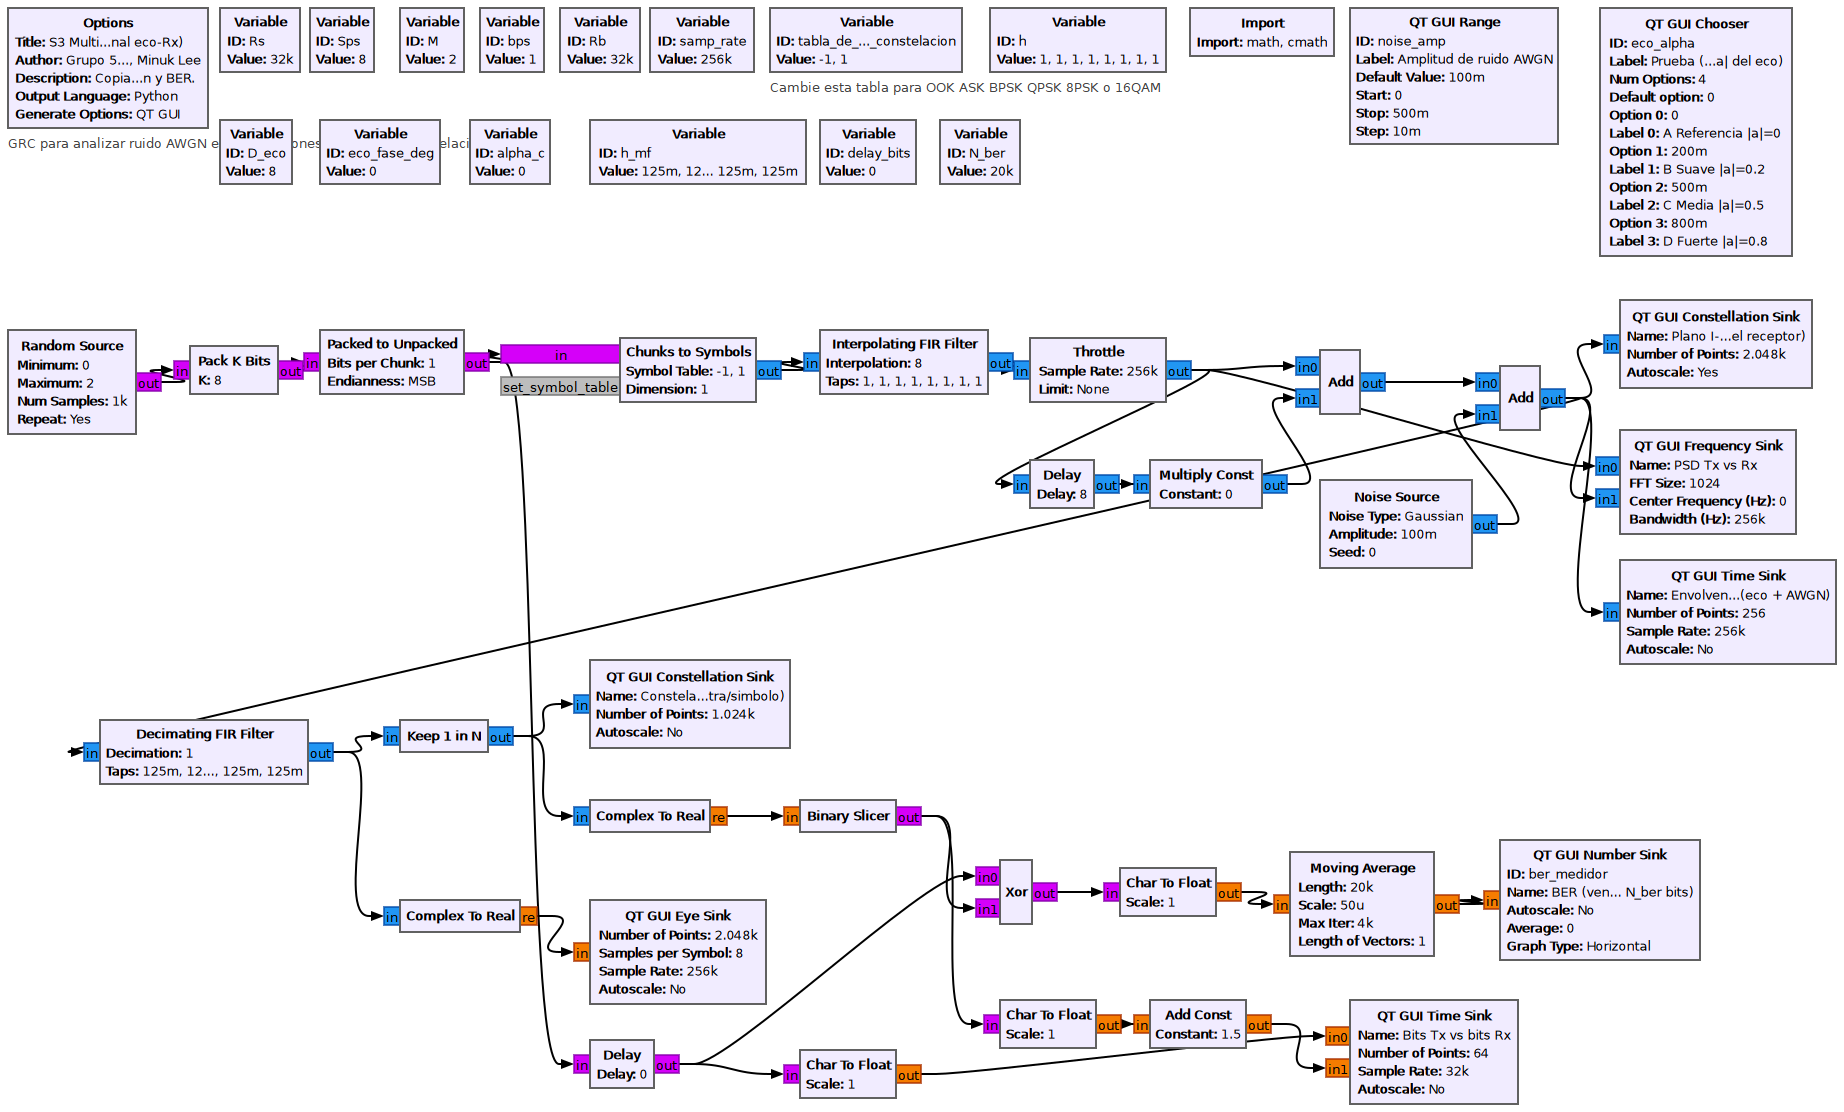
\includegraphics[width=0.92\textwidth]{GRC_S3_Multitrayectoria_BPSK_Grupo5.png}
\caption{GRC modificado \texttt{S3\_Multitrayectoria\_BPSK\_Grupo5.grc} (captura de pantalla de GRC~3.10.12 en el equipo del grupo): Tx BPSK, canal eco (Delay + Multiply Const + Add), AWGN y receptor.}
\label{fig:grc_mod}
\end{figure*}

\subsection{Procedimiento experimental}
Se realizaron cuatro pruebas cambiando solo $|\alpha|$ (Tabla~\ref{tab:pruebas}); $\tau$, la fase, el ruido, $R_s$, $Sps$ y $f_s$ se mantuvieron constantes. Para exportar datos se generó una variante sin GUI del mismo flujograma, en la que los sinks QT se sustituyen por \emph{File Sinks} y el Throttle por un \emph{Head} de 200\,000 bits. Esa variante se ejecutó con GNU Radio 3.10.9 en Linux, y las gráficas se obtuvieron de los datos crudos. El GRC con GUI se ejecutó además en GNU Radio 3.10.12 (radioconda, Windows) en el equipo del grupo, con resultados visuales idénticos (Anexo~\ref{app:evidencias}).

\subsection{Instrumentación BER (Fase 4)}
Se integraron \texttt{e\_EbN0\_Sweep} y \texttt{e\_BER\_Curve} \cite{guia4} en \texttt{S3\_BER\_Multitrayectoria\_BPSK\_Grupo5.grc}. El barrido reemplaza a la fuente AWGN fija y se ubica justo antes del filtro acoplado, con $bb\_rate=f_s=256$~kS/s y $R_b=32\,000$~b/s. La referencia Tx se toma de los bits antes del mapeo, y los bits Rx a la salida del \emph{Binary Slicer}. El ruido agregado cumple
\begin{equation}
    P_n=\frac{P_s\,f_s}{R_b\,(E_b/N_0)},
    \label{eq:pn}
\end{equation}
donde $P_s$ es la potencia medida a la entrada del barrido, que incluye el eco: $P_s=1+|\alpha|^2+2|\alpha|\rho_1$, con $\rho_1$ la correlación entre símbolos adyacentes. La BER teórica de referencia, obtenida de \eqref{eq:yk} y \eqref{eq:pn} con $\rho_1\approx0$, es
\begin{equation}
    P_b=\tfrac12 Q\!\left(\!\sqrt{\tfrac{2\gamma}{P_s}}(1+|\alpha|)\!\right)+\tfrac12 Q\!\left(\!\sqrt{\tfrac{2\gamma}{P_s}}(1-|\alpha|)\!\right),
    \label{eq:pb}
\end{equation}
con $\gamma=E_b/N_0$; para $\alpha=0$ se reduce a $Q(\sqrt{2\gamma})$ \cite{proakis2008}. Se usaron $E_bN_0\in[0,14]$~dB en pasos de 1~dB, \texttt{bits\_por\_punto}$=100\,000$, \texttt{bits\_guardia}$=1000$ y dos barridos completos por cada $|\alpha|$.

Al integrar la plantilla se encontraron y corrigieron dos errores que impedían usarla en GNU Radio 3.10, comprobados en GRC~3.10.12 del equipo (Anexo~\ref{app:correcciones}): (i) \texttt{e\_BER\_Curve} heredaba de \texttt{gr.sync\_decimator}, que en 3.10 es la clase C++ enlazada y no una clase de bloque Python, por lo que GRC no reconoce el bloque; se cambió a \texttt{gr.decim\_block}; (ii) \texttt{e\_BER\_CSV} usa \texttt{\_\_file\_\_}, que no existe cuando GRC instancia el bloque para validarlo; se añadió un respaldo a \texttt{Path.cwd()}. Además, se ligaron los parámetros de \texttt{e\_BER\_Curve} a las variables (\texttt{delay\_bits}, etc.), que en la plantilla no estaban conectados.

\textbf{Alineación Tx/Rx.} En condición limpia (prueba A, $E_b/N_0\approx29$~dB) se evaluó la BER para \texttt{delay\_bits}$=0\ldots8$. Solo con \texttt{delay\_bits}$=0$ se obtuvo BER $=0$ (0 errores en 200\,000 bits); para los demás valores la BER es $\approx0{,}5$. Esto es coherente con la temporización: el filtro acoplado y la decimación no introducen retardo entero de símbolo.

\subsection{Preparación para hardware (Fase 3)}
Se generaron \texttt{S3\_BPSK\_Grupo5\_HackRF\_TX/RX.grc} con los bloques \emph{Osmocom Sink/Source} del archivo de referencia del curso (fc$=960$~MHz, LO desplazado 200~kHz, \texttt{radio\_rate}$=2$~MS/s). La adaptación de tasa es $radio\_rate=bb\_rate\cdot125/16$ y la inversa en Rx, sin cambiar $R_s$. Se retiró el Throttle. Como el hardware no garantiza sincronismo, el Rx incorpora AGC, \emph{Symbol Sync} (Gardner) \cite{gnuradio_symsync} y lazo de Costas de orden~2. Esta cadena se verificó en simulación con desfases de 0 a 3~kHz, error de reloj de 0 a 100~ppm y ruido, y en todos los casos se obtuvieron 0 errores en 100\,000 bits, con la ambigüedad de fase de $180^\circ$ propia de BPSK (bits invertidos), que debe resolverse con una secuencia conocida o con codificación diferencial. La configuración no se probó con hardware porque el radio no estaba disponible.
